% Algoritmos y Complejidad IST 4310
% NRC: 3265
% Name: David Daniel Henriquez Leal
% Student code: 200157506
% Date: 16/11/2022
%
% Sinposis;
% Article that compare the results of using diferent Algorithm Design Techniques
% in the solution of finding the closest pair problem.

%define the article style
\documentclass[journal,onecolumn]{IEEEtran}

%imports required packages

%adds support for embedding graphics
\usepackage{graphics}
\usepackage{graphicx}

%adds support for captions in graphics
\usepackage{caption}

%adds support for mathematical equations
\usepackage{amsmath}

%adds support for displaying algorithms
\usepackage{algorithm}
\usepackage{algorithmic}

%adds support for controlling placement of floats (figures, tables, etc.)
\usepackage{float}	

%adds support for hyperlinks
\usepackage[colorlinks=true, linkcolor=blue, citecolor=blue]{hyperref}

\begin{document}

%creates the title
\title{Divide and Conquer \& Brute Force: Closest Pair}
\author{David~Henriquez, {Estudiante~UNINORTE}}% 
\markboth{Divide and Conquer \& Brute Force: Closest Pair, November 02/2022}%
{}
\maketitle

%input of content from tex files
\begin{abstract}
Existen diferentes técnicas para el diseño de algoritmos que permiten solucionar problema de diversas maneras, cada una teniendo sus ventajas y desventajas. La elección de una de estas técnicas puede ser un trabajo difícil de realizar pues está a criterio del programador priorizar la complejidad espacial, temporal o la facilidad en la comprensión del código, además de que la eficiencia de la técnica depende del problema. Con el fin de facilitar el aprendizaje de cómo tomar esta decisión, realizamos un experimento en el cual solucionamos un problema usando dos técnicas distintas y comparamos sus resultados, para posteriormente determinar cuál de ambas es más eficiente y por ende la metodología que se debe tomar para el programa.
\end{abstract}

% Note that keywords are not normally used for peerreview papers.
\begin{IEEEkeywords}
Algoritmos, eficiencia algoritmica, complejidad temporal, tecnicas para el diseño de algoritmos.
\end{IEEEkeywords}

\IEEEpeerreviewmaketitle
\section{Introducción}
\IEEEPARstart{U}{n} algoritmo es un procedimiento para resolver un problema en particular en una serie de pasos dado unos datos de entrada finitos, estos algoritmos se pueden de diseñar de diversas maneras dependiendo de la creatividad y las ideas de la persona que los realice, sin embargo, existen algunas técnicas de diseño que dan una base sobre la cual desarrollarlo enfocando el problema desde diferentes puntos de vista lo que hace que se resuelvan de diferentes maneras, cada una teniendo sus ventajas y desventajas dependiendo cual sea el problema, pues no hay una estrategia que sea mejor que otra en todos los casos. Dos de las técnicas más comunes en el diseño de algoritmos son “divide y vencerás” y “fuerza bruta o búsqueda exhaustiva”. \cite{DesignTechniques} \\

Divide y vencerás parte de un concepto del cual precede su nombre, pues se basa en seguir tres pasos, primero dividir el problema en sub-problemas más pequeños, luego “conquistar” estos problemas llamándolos de manera recursiva hasta que todos se solucionen y por último combinar todos los sub-problemas para conseguir la solución final del problema principal. Esta técnica reduce la complejidad temporal de la solución de los problemas y usa de manera más eficiente la memoria cache sin ocupar demasiado espacio, sin embargo esta eficiencia depende de la manera en la que se implemente la lógica, en algunos casos la recursividad puede ser lenta y el concepto puede ser algo complejo de aplicar para algunos problemas. \cite{DivideAndConquer}\\

Fuerza bruta parte de un concepto más simple e intuitivo de resolución de problemas, en donde todas las soluciones y caminos posibles son considerados para posteriormente encontrar la solución del problema principal, lo que garantiza que se encontrar la solución correcta, pues enlista todas las posibles soluciones. A pesar de que el concepto sea sencillo de entender y aplicar, utilizar este método suele ser ineficiente, pues suelen tener una complejidad temporal demasiado alta, y requerir mayores recursos que un algoritmo que usan una técnica de diseño más adecuada para el problema. \cite{BruteForce}\\

En este experimento vamos a determinar cuál de estas dos técnicas para el diseño de algoritmos es más eficiente para resolver el problema de encontrar el par de puntos más cercanos en un arreglo ordenado.
\section{Definición del problema}

Se debe realizar un programa en java capaz de crear una lista de N nodos con coordenadas (X, Y) y ordenarlos de forma ascendente, para posteriormente encontrar cual es el par de coordenadas más cercanas usando dos métodos distintos, el método “Divide y vencerás” y el método de “Fuerza bruta”. Por último, se deben tomar datos del número de iteraciones y el tiempo de ejecución para diferentes N en ambos métodos, y de esta manera poder graficarlos y determinar las diferencias en el comportamiento de ambos métodos.
\section{Metodologia}
Para llevar a cabo este programa, primero diseñamos un algoritmo para realizar la búsqueda del par más cercano por medio de la tecnica de fuerza bruta y posteriormente diseñamos un algoritmo recursivo que usa la tecnica de “divide y vencerás” que realiza la misma función que el método anterior.
\begin{algorithm}[H]	
\caption{FuerzaBruta}	
\begin{algorithmic}
\FOR{i = 1, Lista.size - 1}
\FOR{j = 1, Lista.size - 1}
\STATE NodoA = Lista.get(i)
\STATE NodoB = Lista.get(j)
\STATE distX = NodoB.x - NodoA.x
\STATE distY = NodoB.y - NodoA.y
\STATE dist = distX * distX + distY * distY
\IF{dist $<$ DistanciaMinima}
\STATE PrimerNodo = NodoA
\STATE SegundoNodo = NodoB
\STATE DistanciaMinima = dist
\ENDIF
\ENDFOR
\ENDFOR
\end{algorithmic}
\label{algo:factorial}	
\end{algorithm}

\begin{algorithm}[H]	
\caption{DivideYVenceras}	
\begin{algorithmic}
\IF{Lista.size $<=$ 3}
\STATE FuerzaBruta(Lista)
\ELSE
\STATE DivideYVenceras(Primera mitad de la lista)
\STATE DivideYVenceras(Segunda mitad de la lista)
\STATE FuerzaBruta(Medio de la lista)
\ENDIF
\end{algorithmic}
\label{algo:factorial}	
\end{algorithm}

Posteriormente implementamos estos algoritmos en un programa en java y además le agregamos la funcionalidad de contar el número de iteraciones que le toma a cada uno de los métodos realizar su función y el tiempo de ejecución requerido para este. Para la tecnica de divide y venceras el tiempo de ejecución y las iteraciones son calculados a partir del promedio de  6 ejecuciones con el mismo valor de N, pues los resultados son variables dependiendo de los datos y es adecuado realizar este promedio para que los resultados mas precisos.

Por último, con todas las funcionalidades ya implementadas, realizamos pruebas utilizando puntos con coordenadas iguales en ambos métodos, guardamos los datos y repetimos el proceso aumentando el tamaño N para visualizar el comportamiento de estas metodologías cuando N tiende a infinito.
\section{Resultados}
Despues de realizar el experimento el script the python nos arrojo las siguientes graficas:
\begin{figure}[H]
    \centering   
    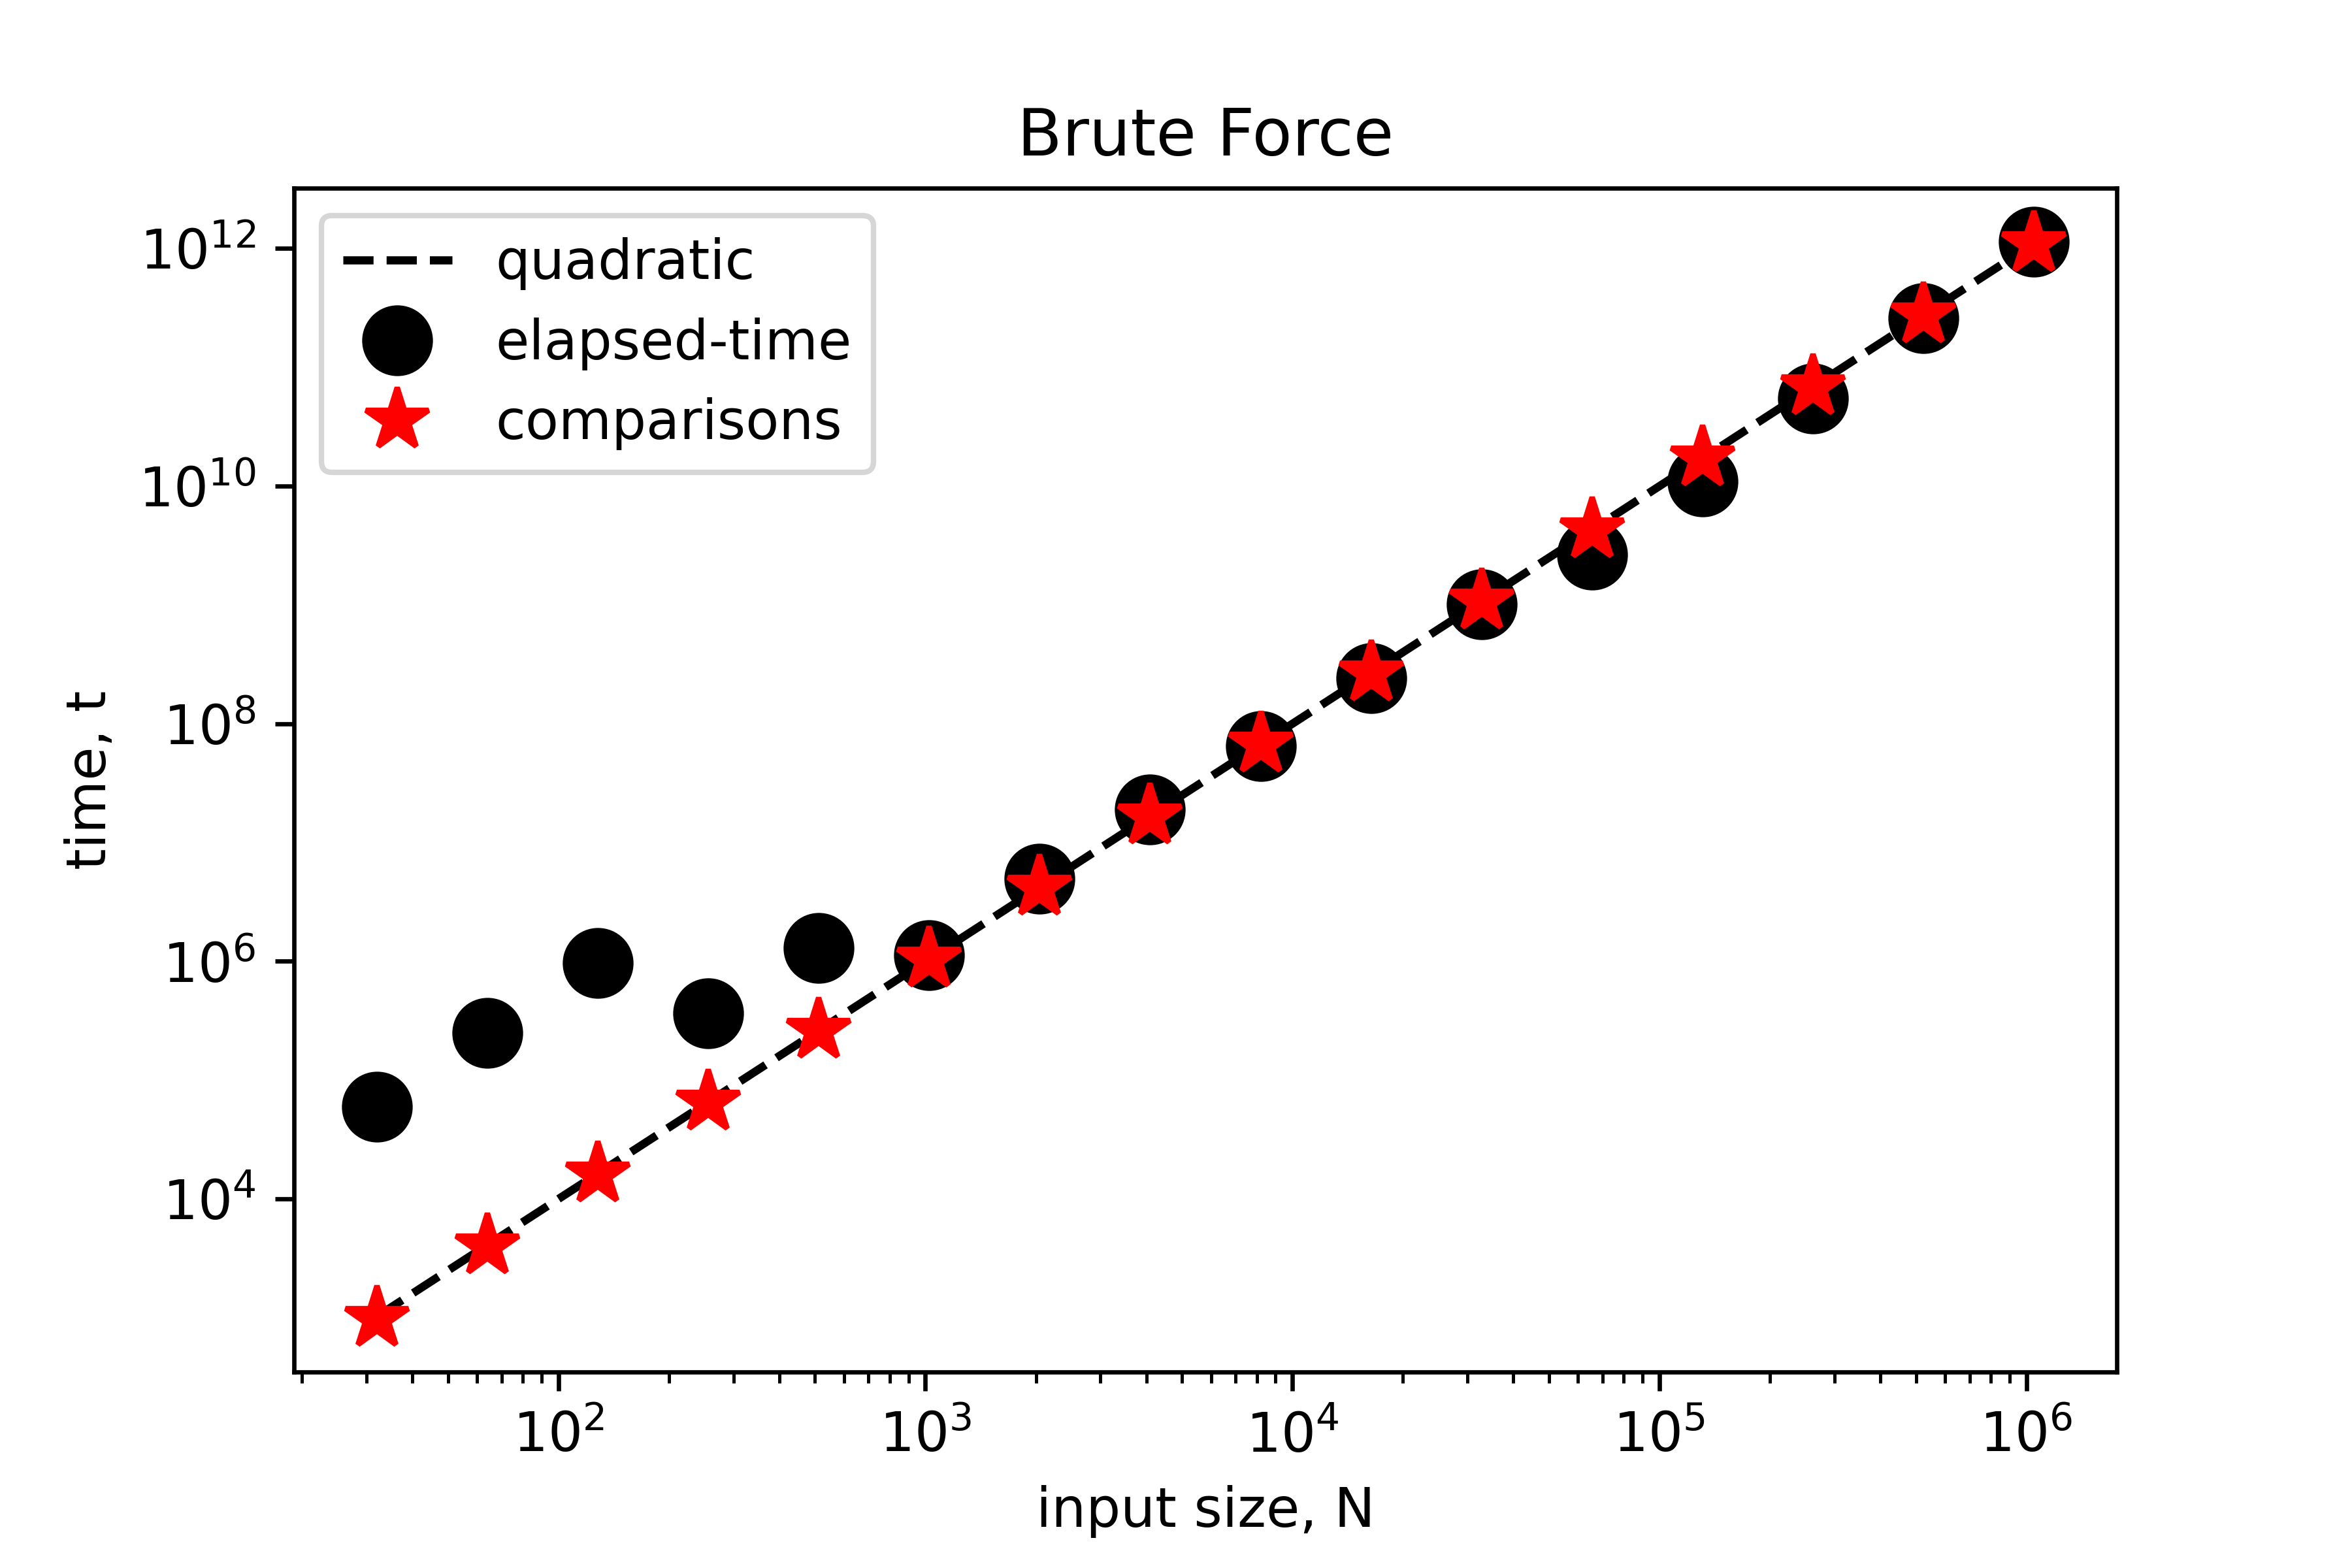
\includegraphics[width=0.45\textwidth,\keepaspectratio]{Images/Brute.png}
    \caption{Comportamiento de la tecnica de Fuerza bruta}
\end{figure}%

\begin{figure}[H]
    \centering    
    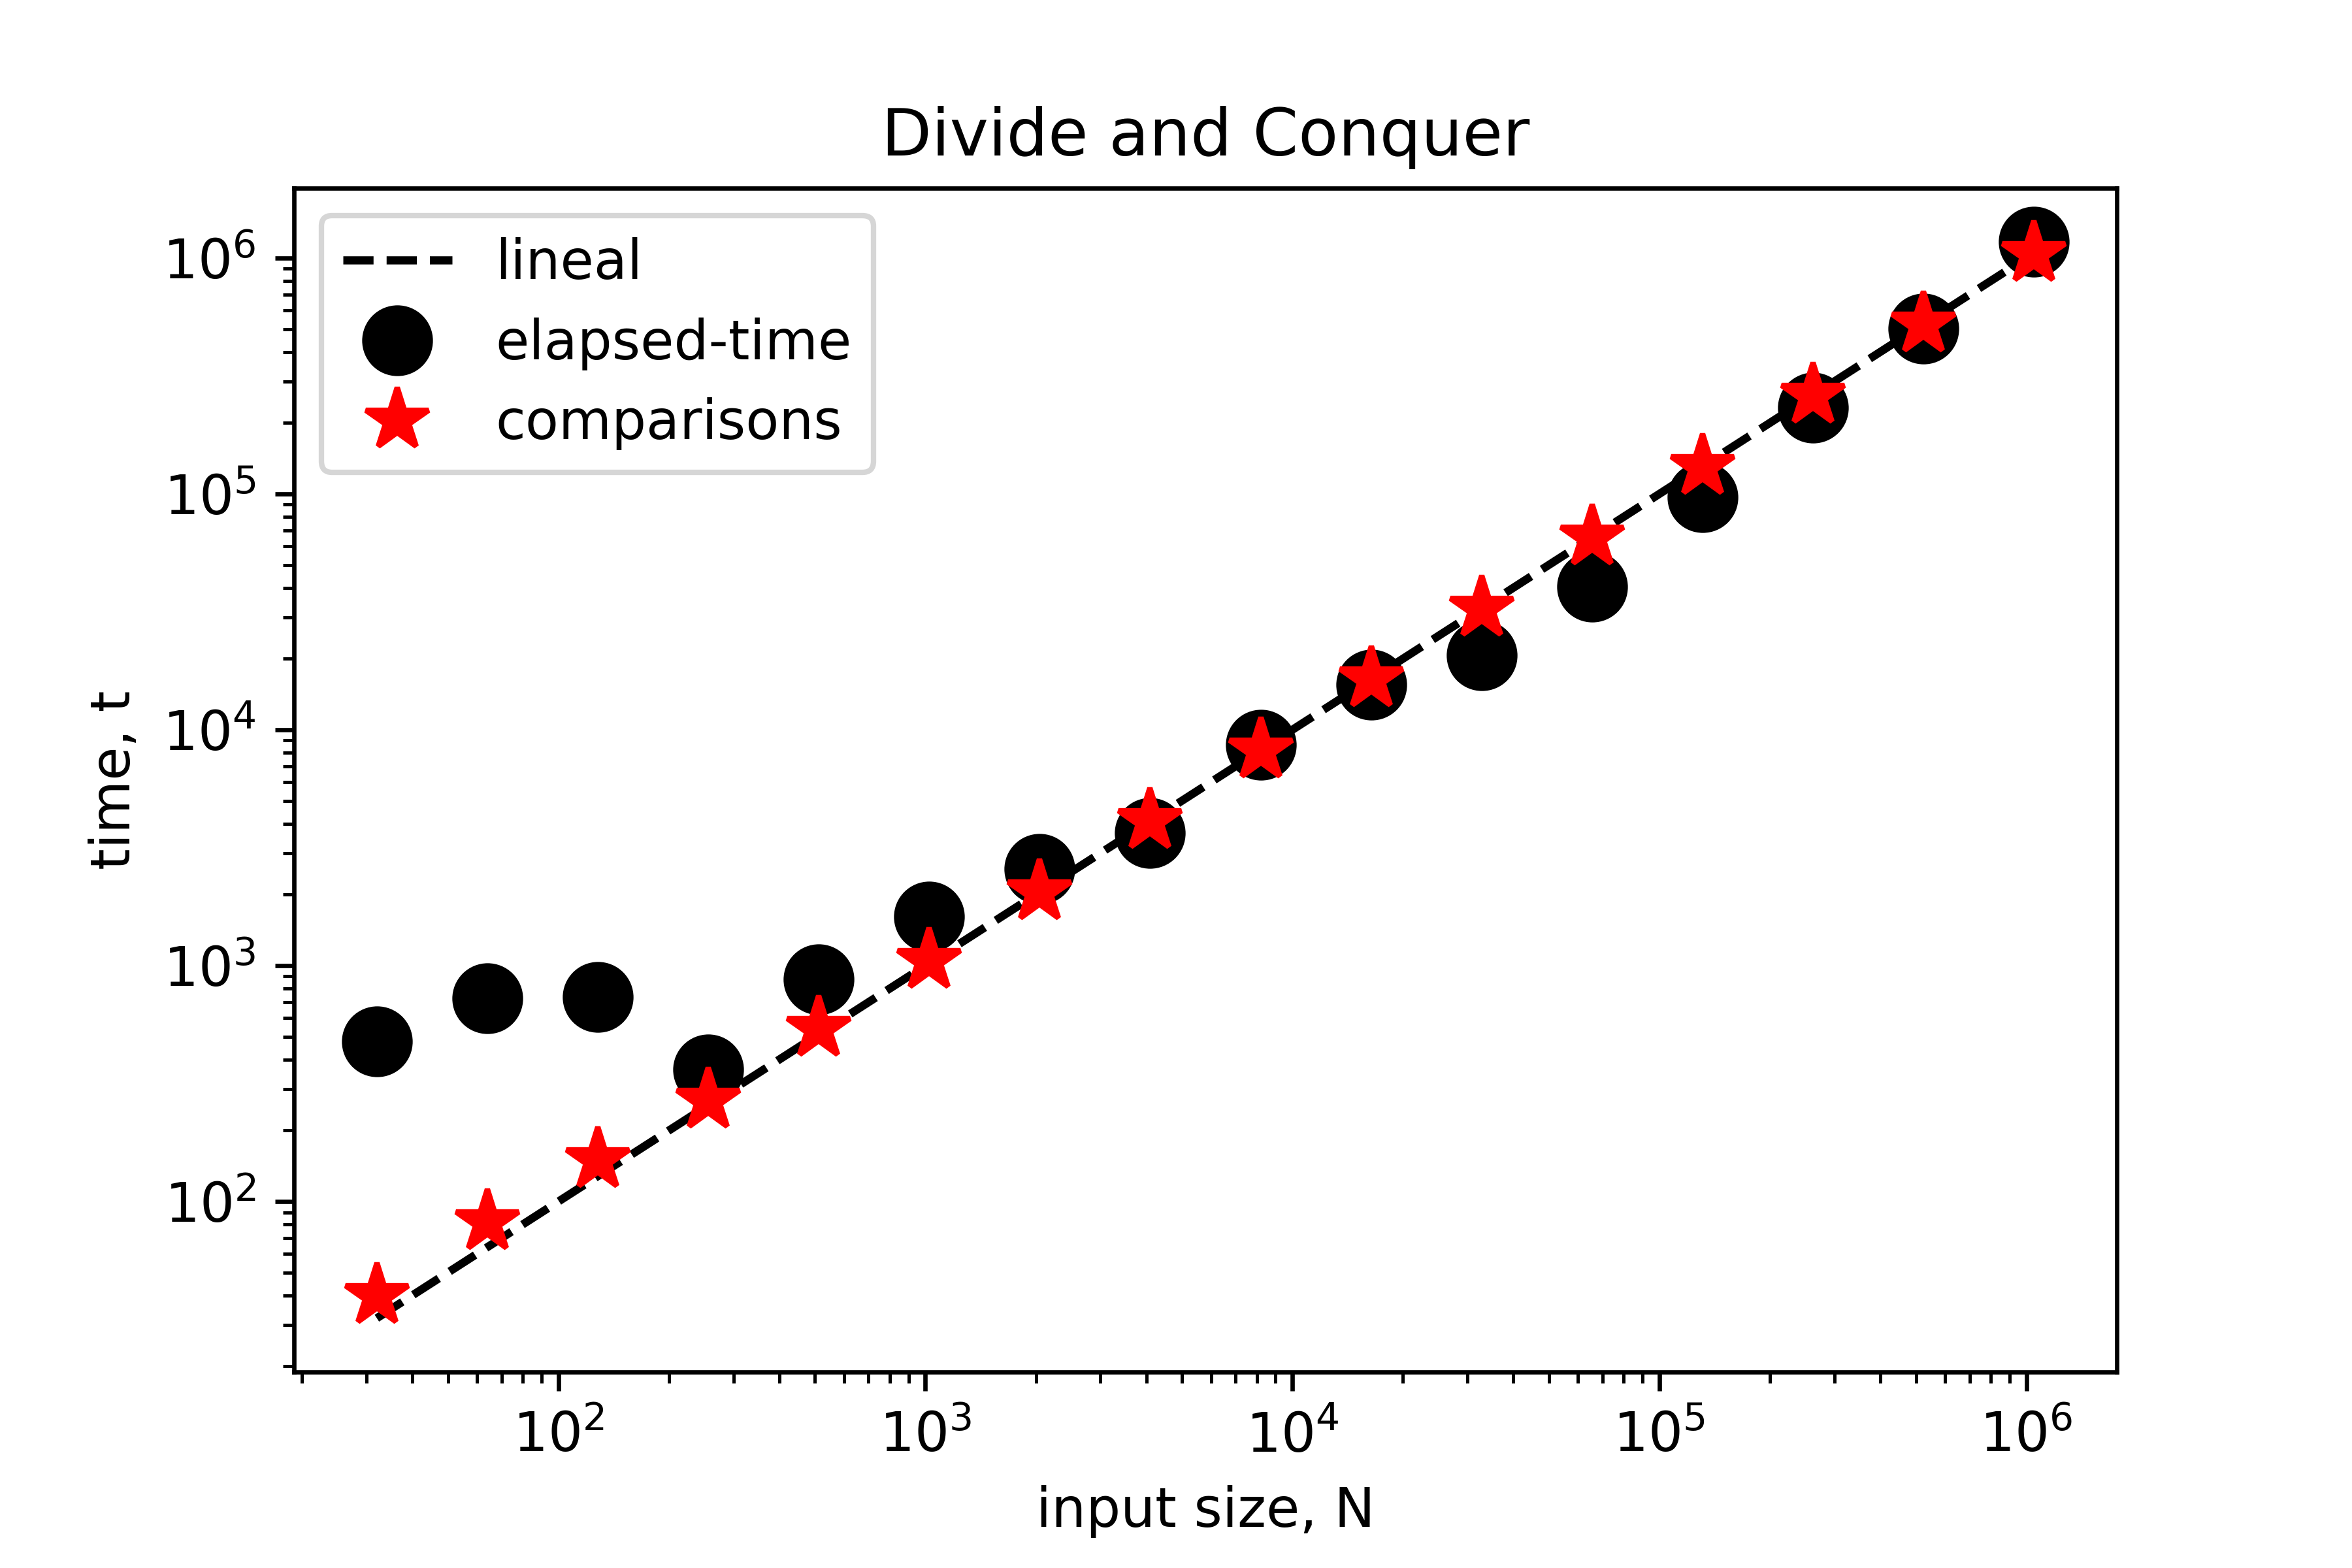
\includegraphics[width=0.45\textwidth,\keepaspectratio]{Images/Divide.png}
    \caption{Comportamiento de la tecnica de Divide y Venceras}
\end{figure}%

Observando las gráficas podemos notar que usando la técnica de “divide y vencerás” la complejidad temporal crece de manera lineal $O(N)$, aunque no de manera totalmente precisa, pues el número de iteraciones depende de la lista de coordenadas, por lo que los datos no están alineados en su totalidad al ajuste lineal, aunque se comportan de manera parecida. Por otro lado, la técnica de “fuerza bruta” tiene una complejidad temporal de $O(N^2)$, es decir que aumenta de manera exponencial, y sin importar los datos del arreglo el número de iteraciones dado un mismo N será el mismo y se ajusta de manera perfecta al ajuste exponencial. La diferencia está en que usando la técnica de “divide y vencerás”, el programa no compara cada par de puntos en la lista, sino que compara solo los que están más cercanos, lo que ahorra una gran cantidad de comparaciones, lo que hace que el número de iteraciones aumenten de manera parecida a N, es decir de manera lineal. Sin embargo, usando la técnica de “fuerza bruta”, sin importar que las coordenadas estén muy lejanas se calcula la distancia entre ellas, lo que hace que se tengan que realizar muchas más comparaciones de las necesarias, y provocan que el número de iteraciones aumenten de manera exponencial a medida que aumente N.
\section{Conclusiones}
Con la realización de este experimento pudimos determinar la importancia de considerar diferentes técnicas para el diseño de algoritmos que deseemos implementar en nuestros programas, con el fin de escoger el que tenga una mayor eficiencia algorítmica, pues notamos en los resultados del experimento que a pesar de que ambas funciones al final retornan lo mismo, el tiempo de ejecución, el número de iteraciones y la complejidad espacial varían mucho entre ellos, lo que nos permite elegir el que mejor nos convenga. 

Además, pudimos observar que, en la mayoría de los casos, los algoritmos recursivos que siguen la técnica de diseño de “divide y vencerás” son más eficientes tanto temporal como espacialmente que los algoritmos iterativos que usan la técnica de diseño de “fuerza bruta”, pues notamos que en la función recursiva solo se realizan comparaciones que son totalmente necesarias, mientras que en la función iterativa se realizan todas las comparaciones posibles, a pesar de que muchas de estas no sean necesarias y no alteren el resultados.  Esto lo pudimos comprobar en las gráficas realizadas a partir de los resultados del experimento, pues notamos que el algoritmo recursivo tubo una complejidad temporal de $O(N)$ y el iterativo tuvo una complejidad temporal de $O(N^2)$.

Por último, a partir de los resultados de nuestro experimento podemos concluir que los algoritmos que siguen la técnica de diseño de “divide y vencerás” tienen una menor complejidad temporal y espacial, y por ende una mayor eficiencia logarítmica en la solución de ese problema, que los algoritmos iterativos que siguen la técnica de diseño de “fuerza bruta”. 
\bibliographystyle{IEEEtran}
\bibliography{references}

\end{document}